
We present a comprehensive analysis of three neural network architectures' performance on the breast cancer histopathological dataset, examining their effectiveness in handling a relatively small medical imaging dataset (780 images). Our analysis spans model accuracy, class-wise performance, and training dynamics to understand how architectural complexity and transfer learning influence classification performance under data constraints.

\subsection{Model Performance Overview}

We present our analysis through confusion matrices (\cref{fig:confusion_matrix}) and classification metrics (\cref{tab:classification_metrics}), which reveals distinct patterns in how each architecture handles the classification task. ResNet101 demonstrates superior and balanced performance across all classes, while both the Simple CNN and MobileNet show characteristic behaviors reflecting their architectural differences and the challenges of limited training data.

\onecolumngrid
\begin{figure}[h!]
    \begin{minipage}{\textwidth}
        \centering
        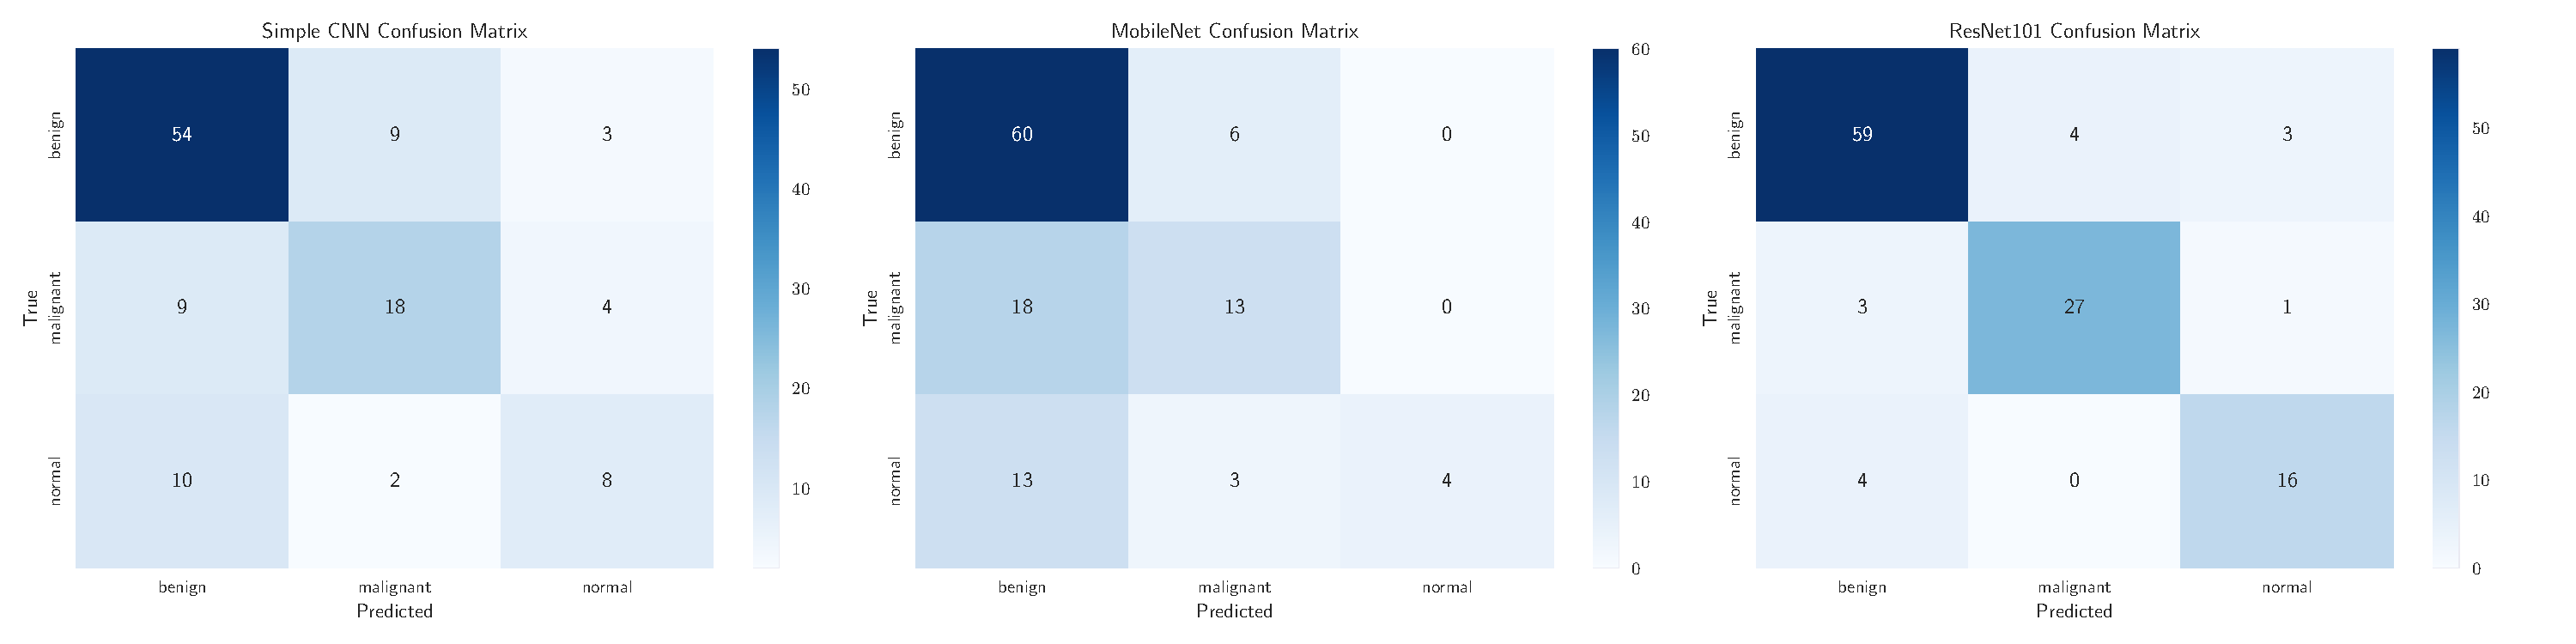
\includegraphics[width = \textwidth]{../figs/confusion_matrices.pdf}
        \caption{Confusion matrices for the three neural network architectures (Simple CNN, MobileNet, and ResNet101) evaluated on the breast cancer histopathological test dataset. Values and color intensity indicate the number of images classified in each category.}
        \label{fig:confusion_matrix}
    \end{minipage}
\end{figure}
\twocolumngrid

The confusion matrices demonstrate distinct classification behaviors across architectures. ResNet101 exhibits balanced prediction distribution across classes, while both the simple CNN and MobileNet display systematic bias toward the majority class (benign), as evidenced by the disproportionate predictions in their respective primary columns.


\begin{table}[h!]
    \centering
    \begin{tabular}{lccc}
        \hline
        & Simple CNN & MobileNet & ResNet101 \\
        \hline
        \multicolumn{4}{l}{\textbf{Precision}} \\
        Benign & 0.74 & 0.66 & 0.89 \\
        Malignant & 0.62 & 0.59 & 0.87 \\
        Normal & 0.53 & 1.00 & 0.80 \\
        \textit{Weighted Avg.} & 0.67 & 0.70 & 0.87 \\
        \hline
        \multicolumn{4}{l}{\textbf{Recall}} \\
        Benign & 0.82 & 0.91 & 0.89 \\
        Malignant & 0.58 & 0.42 & 0.87 \\
        Normal & 0.40 & 0.20 & 0.80 \\
        \textit{Weighted Avg.} & 0.68 & 0.66 & 0.87 \\
        \hline
        \multicolumn{4}{l}{\textbf{F1-score}} \\
        Benign & 0.78 & 0.76 & 0.89 \\
        Malignant & 0.60 & 0.49 & 0.87 \\
        Normal & 0.46 & 0.33 & 0.80 \\
        \textit{Weighted Avg.} & 0.68 & 0.62 & 0.87 \\
        \hline
    \end{tabular}
    \caption{Classification metrics grouped by metric type, comparing performance across models. The weighted averages account for class imbalance in the dataset.}
    \label{tab:classification_metrics}
\end{table}

ResNet101 shows markedly superior behavior compared to both other models, achieving not just higher but more consistent performance across all classes. The confusion matrix demonstrates balanced prediction patterns: correctly identifying 59/66 benign, 27/31 malignant, and 16/20 normal cases. This balanced performance suggests that the pre-trained features, developed on a large diverse dataset, provide a robust foundation that can be effectively fine-tuned even with limited medical imaging data.

The Simple CNN, despite its basic architecture, demonstrates more balanced performance across classes than MobileNet, though with lower overall accuracy. Its confusion matrix reveals consistent prediction patterns, correctly identifying 54 of 66 benign cases (0.82 recall) while maintaining modest but balanced performance on minority classes (malignant: 18/31, normal: 8/20 correct identifications). This suggests that simpler architectures might be more robust to class imbalance when training data is limited, possibly due to fewer parameters needing optimization and thus less opportunity for overfitting to the majority class.

Of particular note is MobileNet's handling of the normal class, where it shows perfect precision (1.00) but poor recall (0.20). This seemingly contradictory result stems from the model's extreme conservatism in predicting the normal class: out of 117 test cases, it only predicted "normal" 4 times. While all of these predictions were correct (hence the perfect precision), the model failed to identify 16 out of 20 normal cases, instead classifying them primarily as benign (13 cases) or malignant (3 cases). This behavior suggests that despite our data augmentation efforts, MobileNet struggled with the class imbalance in the training data, adopting an overly conservative strategy for the minority class.

\onecolumngrid
\subsection{Architectural Performance Analysis }

\begin{figure}[h!]
    \begin{minipage}{\textwidth}
        \centering
        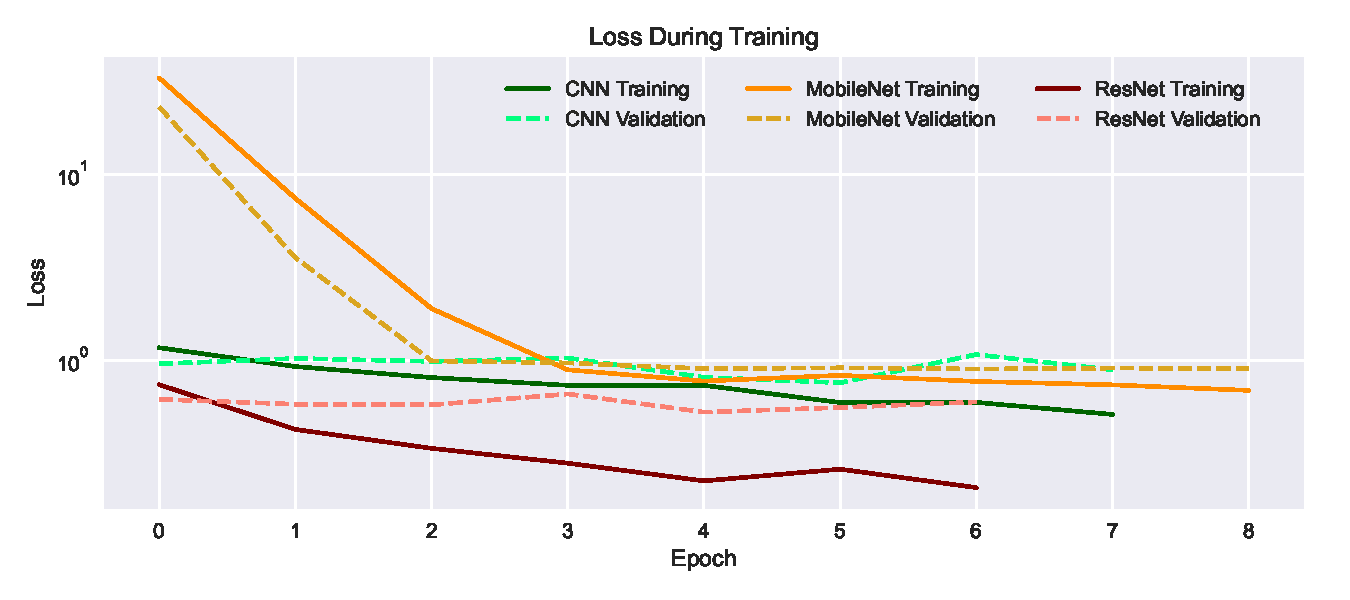
\includegraphics[width = \textwidth]{../figs/cnn_loss.pdf}
        \caption{Loss values during model training plotted on a logarithmic scale. Solid lines represent training loss and dashed lines represent validation loss for each architecture over training epochs.}
        \label{fig:loss_curves}
    \end{minipage}
\end{figure}

\begin{figure}[h!]
    \begin{minipage}{\textwidth}
        \centering
        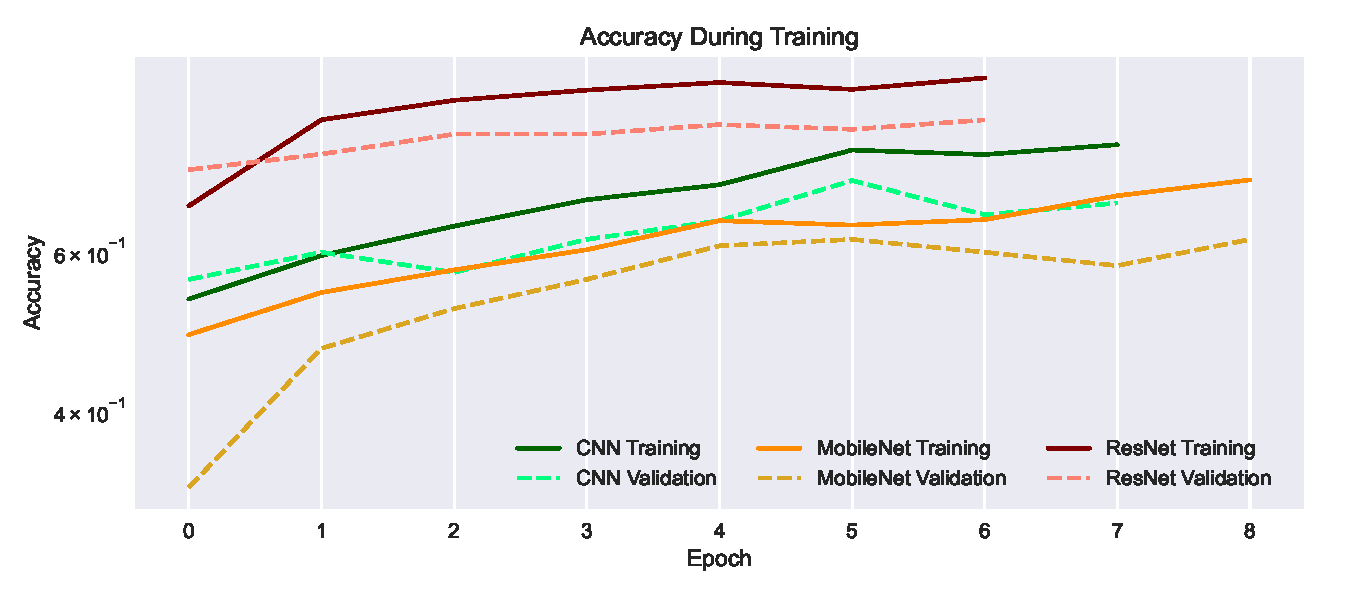
\includegraphics[width = \textwidth]{../figs/cnn_accuracy.pdf}
        \caption{Model accuracy during training. Solid lines show training accuracy and dashed lines show validation accuracy for each architecture over training epochs.}
        \label{fig:accuracy_curves}
    \end{minipage}
\end{figure}
\twocolumngrid

The training dynamics of each model architecture (\cref{fig:loss_curves} and \cref{fig:accuracy_curves}) provide additional insight into model convergence and learning efficiency. ResNet101 initiated training with lower loss values (0.74) compared to the Simple CNN (1.17) and MobileNet (33.19), attributable to its pre-trained weights. The convergence trajectories also differ significantly: ResNet101 exhibited steady descent to a final loss of 0.23, while MobileNet required several epochs to stabilize from its initially high loss values. The Simple CNN maintained intermediate loss values throughout training, converging to 0.59.

Accuracy measurements correlate with these observations. ResNet101 achieved initial validation accuracy of 0.74, improving to 0.83 through training. In contrast, the Simple CNN and MobileNet started at 0.56 and 0.33 respectively, with final validation accuracies of 0.72 and 0.60. Early stopping activated at 7-8 epochs across all architectures, and the proximity between validation and training curves suggests minimal overfitting in all cases. This rapid convergence indicates that performance limitations stem from architectural and data constraints rather than insufficient training duration.
